% !TEX program = xelatex
\documentclass[UTF8,12pt,a4paper,fontset=fandol]{ctexart}

\usepackage[a4paper,top=2.5cm,bottom=2.5cm,left=2.5cm,right=2.5cm]{geometry}
\usepackage{amsmath,amssymb,bm,mathtools}
\usepackage{graphicx}
\usepackage{float}
\usepackage{needspace,placeins}
\usepackage{booktabs,array,longtable,tabularx,multirow}
\usepackage{siunitx}
\usepackage{xcolor}
\usepackage{listings}
\usepackage{hyperref}
\usepackage{titlesec}
\usepackage{tocloft}
\usepackage{caption}
\usepackage{enumitem}
\usepackage{tikz}
\usetikzlibrary{arrows.meta,positioning,fit,calc}

\graphicspath{{figures/}}
\sisetup{detect-all,per-mode=symbol}
\linespread{1.43}
\setlength{\parindent}{2em}
\setlength{\parskip}{0pt}
\setlist{nosep,leftmargin=2.2em}
\captionsetup{font=small,labelsep=quad}
\hypersetup{hidelinks}
\numberwithin{equation}{section}

\ctexset{
  section/number       = \arabic{section},
  subsection/number    = \arabic{section}.\arabic{subsection},
  subsubsection/number = \arabic{section}.\arabic{subsection}.\arabic{subsubsection}
}

\titleformat{\section}
  {\centering\fontsize{14pt}{18pt}\heiti\bfseries}
  {\arabic{section}}{1em}{}
\titleformat{\subsection}
  {\fontsize{12pt}{16pt}\heiti\bfseries}
  {\arabic{section}.\arabic{subsection}}{1em}{}
\titleformat{\subsubsection}
  {\fontsize{12pt}{16pt}\heiti\bfseries}
  {\arabic{section}.\arabic{subsection}.\arabic{subsubsection}}{1em}{}

\titlespacing*{\section}{0pt}{14pt}{9pt}
\titlespacing*{\subsection}{0pt}{10pt}{5pt}
\titlespacing*{\subsubsection}{0pt}{8pt}{4pt}
\AddToHook{cmd/section/before}{\FloatBarrier\Needspace{5\baselineskip}}
\AddToHook{cmd/subsection/before}{\Needspace{4\baselineskip}}

\lstset{
  basicstyle=\ttfamily\small,
  backgroundcolor=\color{black!3},
  frame=single,
  breaklines=true,
  showstringspaces=false,
  columns=fullflexible,
  keepspaces=true
}

% 草稿开关：提交前改为 \draftmodefalse。
\newif\ifdraftmode
\draftmodetrue
\newcommand{\draftnote}[1]{%
  \ifdraftmode
    \par\smallskip\noindent
    \fcolorbox{red!65!black}{red!4}{%
      \parbox{0.94\textwidth}{\color{red!65!black}\textbf{待确认：}#1}%
    }\par\smallskip
  \fi
}
\newcommand{\resultblank}[1]{%
  \ifmmode\text{\color{red!65!black}【#1】}%
  \else\textcolor{red!65!black}{【#1】}%
  \fi
}

\newcommand{\papertitle}[1]{%
  \thispagestyle{empty}
  \begin{center}
    {\fontsize{17.3pt}{22pt}\heiti\bfseries #1}
  \end{center}
  \vspace{1em}
}

\newcommand{\abstractcn}[2]{%
  \begin{center}{\fontsize{14pt}{17pt}\heiti\bfseries 摘要}\end{center}
  #1\par
  \vspace{1em}
  {\heiti\bfseries 关键词：}#2\par
  \newpage
}

\newcommand{\placeholderfigure}[2]{%
  \ifdraftmode
  \begin{figure}[H]
    \centering
    \fbox{\parbox{0.78\textwidth}{\centering\vspace{1.8em}#1\vspace{1.8em}}}
    \caption{#2}
  \end{figure}
  \fi
}

\begin{document}
\pagestyle{plain}

\papertitle{药材热风烘干过程中的热湿耦合与收缩效应建模}

\abstractcn{%
本文针对圆柱形中药材的热风烘干过程，围绕预热阶段、全过程干燥、达标时刻判定和尺寸收缩四个递进问题建立模型。

针对问题一，本文根据附件~1 的烘房温湿度边界与附录~2 的材料参数，建立\resultblank{模型名称}，得到 $0$--$1800\,\mathrm{s}$ 内药材径向温度和干基含水率分布。数值结果表明\resultblank{填写最重要的定量结论及验证结果}。

针对问题二，本文从 $t=0$ 重新计算，采用附录~3 的状态相关物性建立固定半径下的热湿耦合模型，并用守恒有限体积与联立 BDF 求解；积分器内部以 $z=\log C$ 保持含水率正性。$3\,\mathrm{h}$ 时中心和表面温度分别为 $49.8495$ 和 $49.9664\,{}^\circ\mathrm{C}$，含水率分别为 $1.7662$ 和 $1.0081\,\mathrm{kg/kg}$；网格与时间加密检验显示表中数值的四位小数稳定。

针对问题三，本文以药材内部最大含水率达到 $0.15\,\mathrm{kg/kg}$ 的临界时刻作为终点，通过 BDF 连续插值上的事件求根得到烘干时长 $57.4722\,\mathrm h$；全过程径向单调性检验表明圆心为控制位置。

针对问题四，本文将实测半径变化引入归一化空间坐标，在移动边界上重建水分输运模型，并通过\resultblank{固定半径/变化半径等控制变量比较}区分尺寸收缩与物性公式变化的作用，得到烘干时长为\resultblank{结果及单位}。

最后，本文从网格与时间步收敛、边界条件、质量平衡和关键参数敏感性等方面验证模型。\resultblank{填写验证结论，避免只写“误差较小”}。
}{%
热湿耦合 \quad 非线性扩散 \quad 数值仿真 \quad 移动边界 \quad 烘干时长
}

\tableofcontents
\newpage

\section{问题重述}

\subsection{问题背景}

热风烘干通过调节烘房温度与湿度，促使药材内部热量传递和水分迁移。工艺参数不当会造成干燥时间延长、内部水分不均或品质波动。题目以长 $25\,\mathrm{cm}$、初始半径 $2\,\mathrm{cm}$ 的近似圆柱形药材为对象，要求利用附件中的环境和尺寸数据，描述其径向温度场与干基含水率场，并确定烘干时间。

\subsection{问题要求}

\begin{enumerate}
  \item \textbf{预热平衡阶段：}利用附件~1 给出的烘房温度和水分浓度变化，以及附录~2 的常物性参数，求 $0$--$1800\,\mathrm{s}$ 内不同径向位置的药材温度和干基含水率，并生成 \texttt{result1.xlsx}。
  \item \textbf{整个烘干过程：}采用附录~3 的含水率、温度相关经验公式，描述预热平衡与恒温干燥阶段的热湿演化，给出前 $3\,\mathrm{h}$ 的规定结果，并生成 \texttt{result2.xlsx}。
  \item \textbf{烘干时长判定：}以药材各处干基含水率均低于 $0.15\,\mathrm{kg/kg}$ 为终止要求，确定首次达标的时间，并生成 \texttt{result3.xlsx}。
  \item \textbf{考虑尺寸变化：}利用附件~2 的药材半径数据和附录~4 的经验公式，将固定区域模型扩展到收缩区域，重新确定烘干时长，并生成 \texttt{result4.xlsx}。
\end{enumerate}

四问的核心递进关系是：问题一建立固定半径下的基础时空求解框架；问题二引入变物性和阶段衔接；问题三在全过程解上增加终点事件判定；问题四进一步改变计算区域和材料参数口径。

\draftnote{附件数据与四个 Excel 模板尚未加入当前工作区。拿到附件后，应核对时间覆盖范围、列名、单位、缺失值以及 result2.xlsx 要求的实际结束时间。}


\section{数据理解与总体框架}

\subsection{数据和参数来源}

表~\ref{tab:data-source} 给出四问所需信息及其用途。题面给出的干基含水率定义为单位干物质质量对应的水质量，后续守恒关系和平均含水率计算必须沿用这一口径。

\begin{table}[H]
  \centering
  \caption{数据、经验公式与模型用途}
  \label{tab:data-source}
  \begin{tabularx}{\textwidth}{p{0.16\textwidth}p{0.30\textwidth}X}
    \toprule
    来源 & 主要内容 & 用途 \\
    \midrule
    题面 & 几何尺寸、初始温度 $28\,{}^\circ\mathrm{C}$、初始含水率 $2.55\,\mathrm{kg/kg}$ & 初始区域和初始条件 \\
    附件~1 & 烘房温度与水分浓度的时间序列 & 表面热、湿边界及阶段划分 \\
    附件~2 & 药材半径随时间的变化 & 问题四的移动边界 $R(t)$ \\
    附件~3 & 四个结果文件模板 & 输出时间、空间网格和工作表格式 \\
    附录~2 & 问题一的常物性和对流参数 & 预热阶段固定参数模型 \\
    附录~3 & 问题二、三的变物性经验公式 & 全过程热湿演化和达标判断 \\
    附录~4 & 问题四的变物性经验公式 & 收缩区域上的热湿演化 \\
    \bottomrule
  \end{tabularx}
\end{table}

\subsection{预处理和统一口径}

附件数据进入模型前统一转换为 SI 单位：半径由厘米换算为米，摄氏温度在经验式中换算为开尔文，时间统一以秒存储、在论文表格中按题目要求换算为小时。离散时间之外的烘房边界和半径通过\resultblank{待选择的插值方法}计算，并检查插值是否引入超出原始范围的振荡。

所有结果先按完整精度计算，再在 Excel 和论文表格的最终输出环节统一保留四位小数。代码输出、结果报告和论文表格使用同一份数据源，避免多次人工复制带来口径差异。

\draftnote{收到附件后补充数据规模、采样间隔、缺失和异常情况。未经 EDA 核对前，不在正文声称数据连续、无异常或满足某种函数形式。}

\subsection{四问的模型递进}

四问的求解顺序如图~\ref{fig:framework} 所示。

% Source: figures/流程图.svg; converted to vector PDF for XeLaTeX.
\begin{figure}[H]
  \centering
  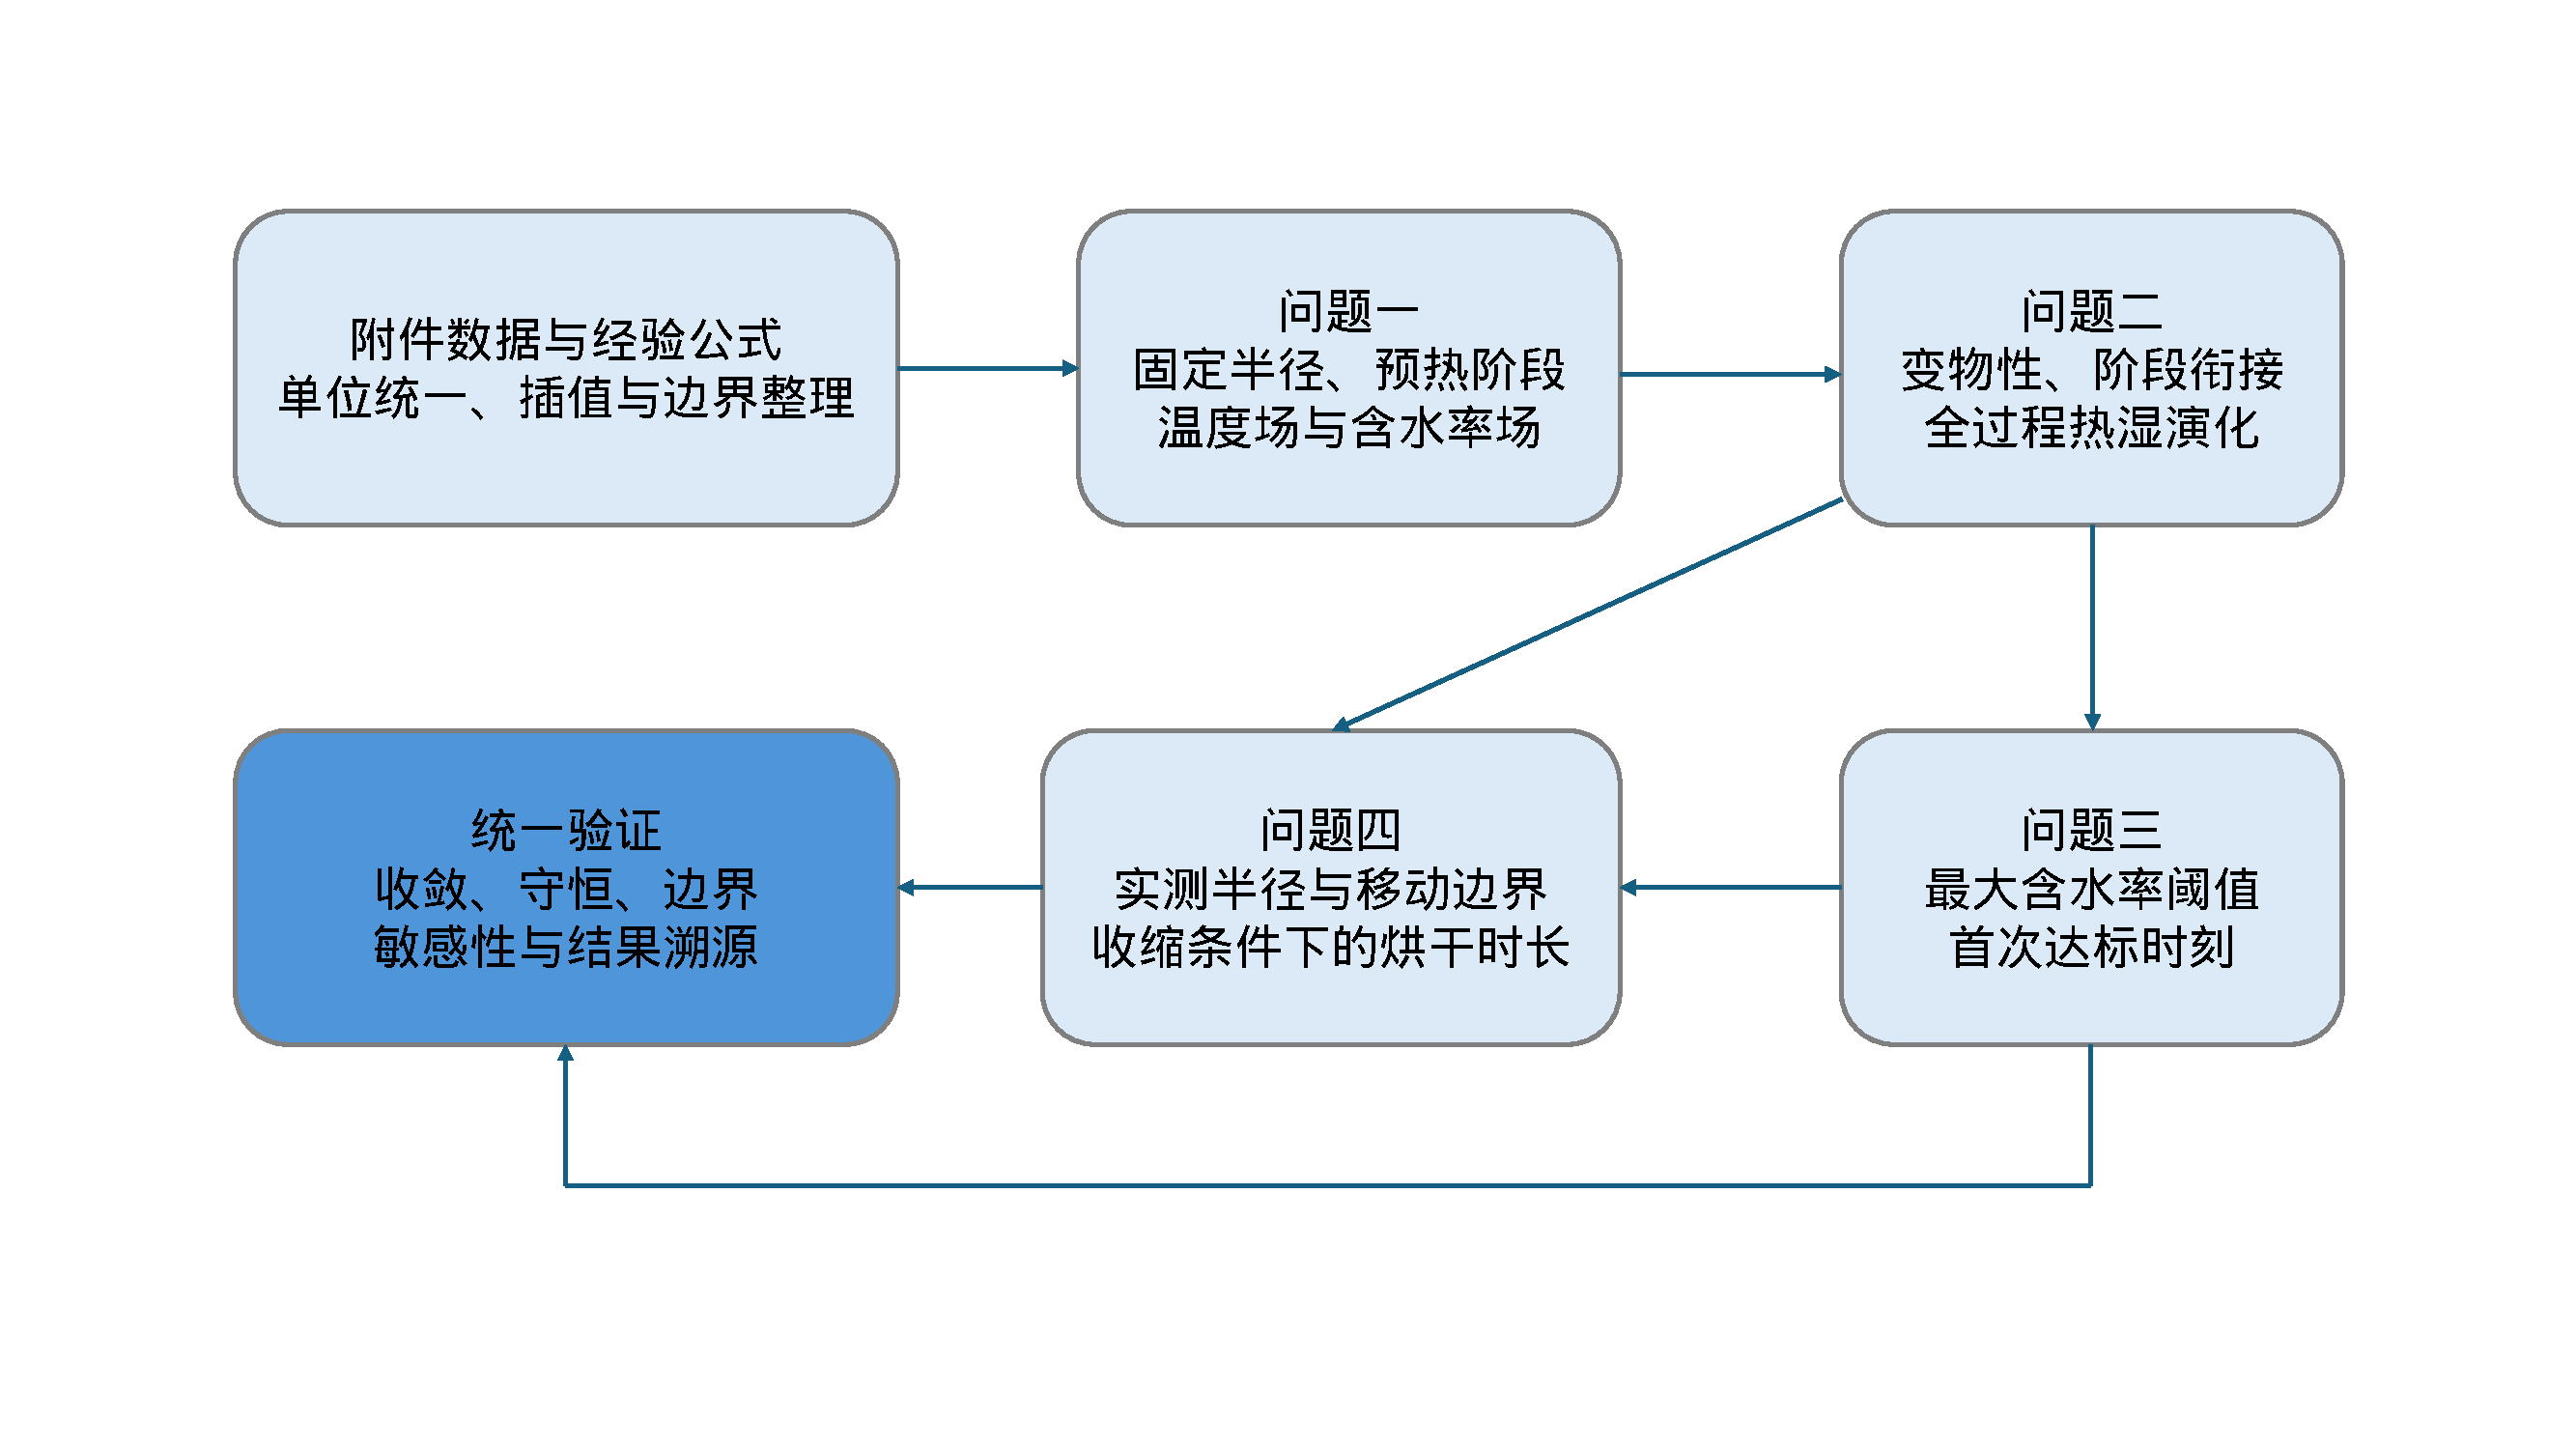
\includegraphics[width=\textwidth]{figures/model_flowchart.pdf}
  \caption{四问建模流程}
  \label{fig:framework}
\end{figure}


问题二是全题的主干：其状态量和数值求解器被问题三直接复用；问题四则复用其热湿传递结构，但必须重写随半径变化的空间处理。问题三与问题四的烘干时长均通过“整个当前药材区域的最大含水率首次低于阈值”判断。

\subsection{论文结果来源约定}

问题一至问题四的关键表格分别由 \texttt{result1.xlsx} 至 \texttt{result4.xlsx} 的同源数据生成。图表用于解释径向梯度、阶段转换、终点附近变化和收缩影响；论文不直接使用临时计算、聊天记录或手工估算的数值。


\section{模型假设}

\begin{enumerate}
  \item 将药材视为连续介质，以有效热物性和扩散系数描述其内部传递过程，不单独分辨细胞、孔隙等微观结构。
  \item 以附件给出的烘房温度与水分浓度代表药材侧壁周围的环境状态，忽略侧壁不同位置的环境差异，表面交换由题目给定的对流参数描述。
  \item 不考虑药材内部化学反应等过程产生的体热源。
  \item 烘干阶段切换时，药材内部温度与含水率连续变化，不因环境边界改变而人为重置。
\end{enumerate}

固定几何、常物性及潜热处理等局部选择在对应小问中说明。题目给定的尺寸、初值和物性参数作为已知条件使用。

\section{符号说明}

本文主要符号如表~\ref{tab:symbols} 所示。下标 $\infty$ 表示烘房环境量，下标 $s$ 表示药材表面量。

\begin{longtable}{>{\centering\arraybackslash}p{0.16\textwidth}p{0.58\textwidth}>{\centering\arraybackslash}p{0.16\textwidth}}
\caption{主要符号说明}\label{tab:symbols}\\
\toprule
符号 & 说明 & 单位 \\
\midrule
\endfirsthead
\toprule
符号 & 说明 & 单位 \\
\midrule
\endhead
$r$ & 到药材中心轴线的径向距离 & $\mathrm{m}$ \\
$t$ & 烘干开始后的时间 & $\mathrm{s}$ \\
$R_0$ & 不考虑收缩时的药材半径，$R_0=0.02$ & $\mathrm{m}$ \\
$R(t)$ & 考虑收缩时的药材半径 & $\mathrm{m}$ \\
$\xi$ & 归一化径向坐标，$\xi=\frac{r}{R(t)}$ & -- \\
$T(r,t)$ & 药材内部温度 & $\mathrm{K}$ 或 ${}^\circ\mathrm{C}$ \\
$C(r,t)$ & 药材内部干基含水率 & $\mathrm{kg/kg}$ \\
$T_\infty(t)$ & 烘房温度 & $\mathrm{K}$ 或 ${}^\circ\mathrm{C}$ \\
$C_\infty(t)$ & 烘房水分浓度 & $\mathrm{kg/kg}$ \\
$\rho(C)$ & 药材密度 & $\mathrm{kg/m^3}$ \\
$c_p(C)$ & 药材比热容 & $\mathrm{J/(kg\cdot K)}$ \\
$k(C)$ & 药材导热系数 & $\mathrm{W/(m\cdot K)}$ \\
$D(C,T)$ & 水分扩散系数 & $\mathrm{m^2/s}$ \\
$h$ & 对流换热系数 & $\mathrm{W/(m^2\cdot K)}$ \\
$h_m$ & 对流传质系数 & $\mathrm{m/s}$ \\
$C_{\mathrm{lim}}$ & 烘干达标阈值，$C_{\mathrm{lim}}=0.15$ & $\mathrm{kg/kg}$ \\
$t_{\mathrm{end}}$ & 药材内部各处首次全部达标的时间 & $\mathrm{s}$ 或 $\mathrm{h}$ \\
\bottomrule
\end{longtable}

\draftnote{温度在偏微分方程中可采用摄氏度，但附录经验式中的 $T$ 明确使用开尔文。代码、符号表和公式应统一命名，并在代入经验式前显式换算。}


\begingroup
\linespread{1.20}\selectfont
\Needspace{0.70\textheight}
\section{模型准备}
\label{sec:model-preparation}

\subsection{控制方程}

热风首先与药材表面交换热量和水分，内部状态再通过热传导与扩散发生变化。以圆柱中心轴为轴线，记径向距离为 $r$、时间为 $t$，温度与干基含水率分别为 $T(r,t)$ 和 $C(r,t)$。以下建立固定区域、忽略端部影响时的径向基础模型；其具体适用范围在各问中说明。

图~\ref{fig:cylinder-shell} 给出了药材截面、薄壳微元及表面交换方向。取半径从 $r$ 到 $r+\mathrm{d}r$、长度为 $L$ 的同轴薄壳，建立径向能量守恒关系。图中颜色用于示意升温和失水后的径向差异。

\begin{figure}[H]
  \centering
  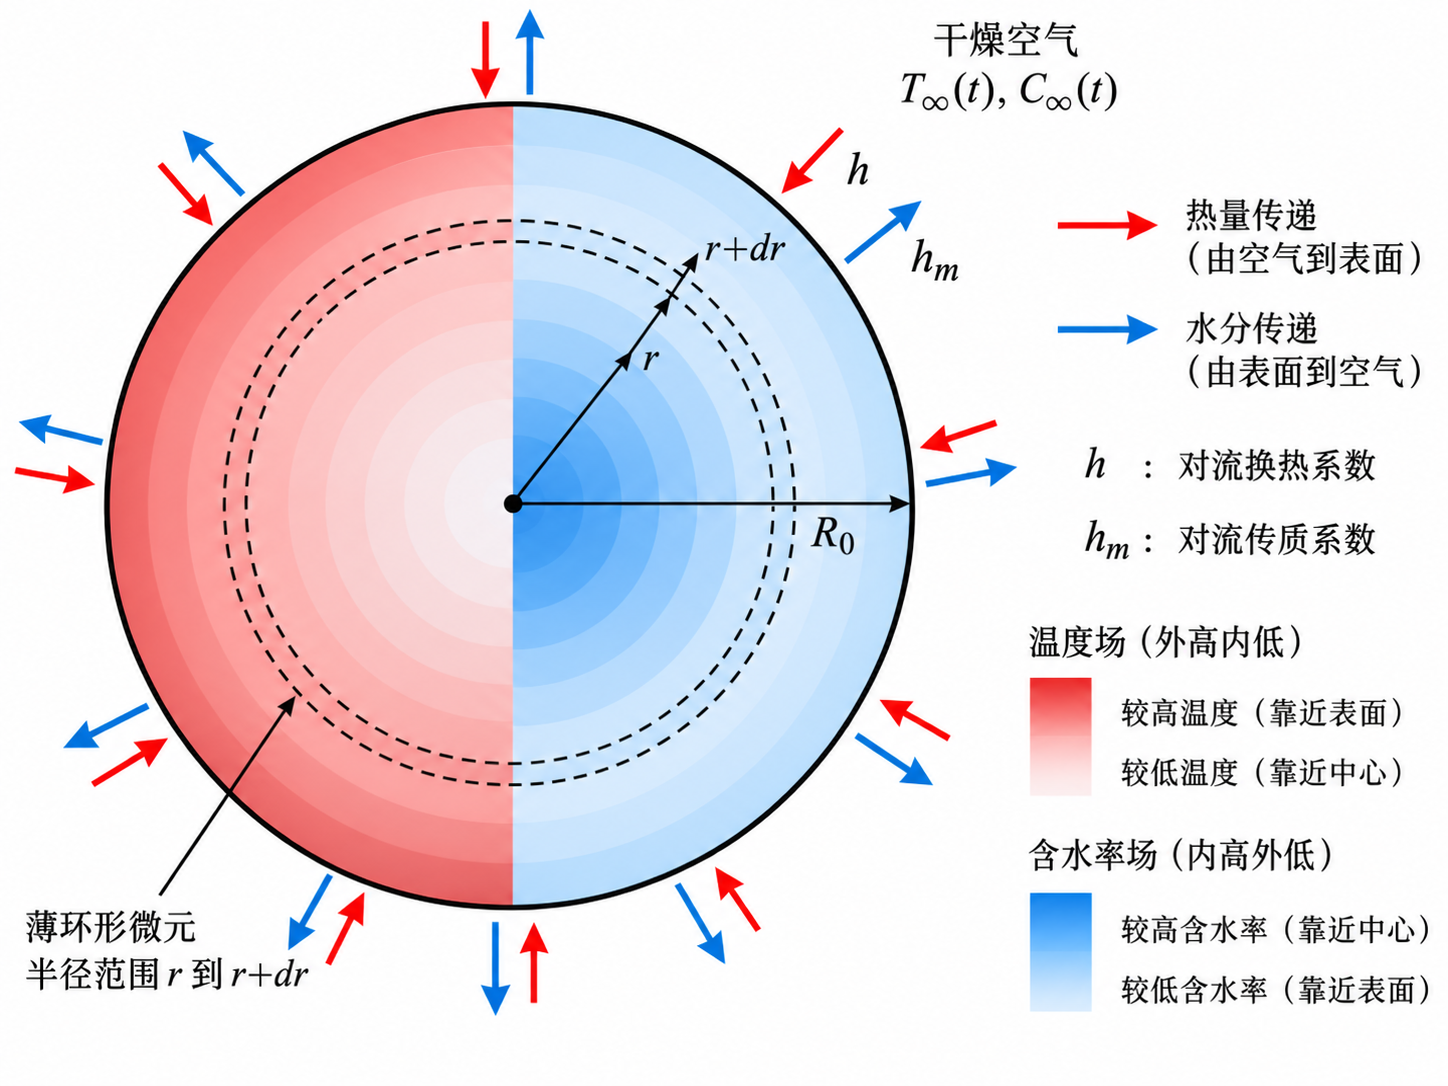
\includegraphics[width=0.90\textwidth]{figures/cylinder_heat_transfer.png}
  \caption{圆柱药材的径向传递及薄壳微元}
  \label{fig:cylinder-shell}
\end{figure}

\noindent\textbf{（1）热传导方程。}根据傅里叶定律，沿半径增大方向通过圆柱面的热流率为

\[
\mathrm{heat}(r,t)
=-2\pi rLk\frac{\partial T}{\partial r}.
\]

取厚度为 $\mathrm{d}r$ 的同轴薄壳，由\textbf{能量守恒}，有

\[
\rho c_p\,2\pi rL\,\mathrm{d}r
\frac{\partial T}{\partial t}
=-\frac{\partial\mathrm{heat}}{\partial r}\,\mathrm{d}r.
\]

代入热流关系并约去公因子，得到圆柱坐标下的一维非稳态热传导方程：

\begin{equation}
\rho c_p\frac{\partial T}{\partial t}
=\frac{1}{r}\frac{\partial}{\partial r}
\left(rk\frac{\partial T}{\partial r}\right),
\qquad 0<r<R_0.
\label{eq:prep-heat}
\end{equation}

式中，$\rho$、$c_p$ 和 $k$ 分别为密度、比热容与导热系数。

\noindent\textbf{（2）水分扩散方程。}将题目所给干基含水率 $C$ 作为有效扩散变量，直接采用圆柱坐标下的 Fick 第二定律：

\begin{equation}
\frac{\partial C}{\partial t}
=\frac{1}{r}\frac{\partial}{\partial r}
\left(rD\frac{\partial C}{\partial r}\right).
\label{eq:prep-moisture}
\end{equation}

$D$ 为有效扩散系数。式~\eqref{eq:prep-heat} 和式~\eqref{eq:prep-moisture} 均\textbf{将物性系数保留在空间微分算子内部}，以便在后续小问中引入状态相关物性；收缩区域还需结合物料运动和区域变化调整输运方程。

\subsection{定解条件}

设初始温度与含水率分别为 $T_0$、$C_0$。均匀初始状态与圆心对称条件写为

\begin{equation}
\left\{
\begin{aligned}
T(r,0)&=T_0,& C(r,0)&=C_0,\\
\left.\frac{\partial T}{\partial r}\right|_{r=0}&=0,
&
\left.\frac{\partial C}{\partial r}\right|_{r=0}&=0.
\end{aligned}
\right.
\label{eq:prep-initial-center}
\end{equation}

记表面状态为 $T_s(t)=T(R_0,t)$、$C_s(t)=C(R_0,t)$，烘房环境量为 $T_\infty(t)$、$C_\infty(t)$。采用对流换热与传质条件：

\begin{equation}
\left\{
\begin{aligned}
-k\left.\frac{\partial T}{\partial r}\right|_{r=R_0}
&=h\left[T_s(t)-T_\infty(t)\right],\\
-D(C_s,T_s)\left.\frac{\partial C}{\partial r}\right|_{r=R_0}
&=h_m\left[C_s(t)-C_\infty(t)\right].
\end{aligned}
\right.
\label{eq:prep-surface}
\end{equation}

其中 $h$、$h_m$ 分别为对流换热和传质系数；若本问的 $D$ 仅与 $C$ 有关，则取 $D(C_s)$。具体物性、环境边界及区域变化在各小问中确定。

\subsection{模型应用}

上述方程构成各问的共同基础。\textbf{第一问}在固定半径、常热物性下计算预热阶段；\textbf{第二问}引入状态相关物性，按本问条件计算全过程，并在阶段切换时延续内部状态；\textbf{第三问}利用第二问的状态演化判定首次全部达标时刻；\textbf{第四问}进一步引入尺寸收缩，调整输运方程、计算区域和表面条件。各问继承同一方程框架，具体物性与区域条件分别确定。

\section{问题一：预热阶段的温度与含水率分布}

\subsection{问题分析}

问题一要求确定前 $1800\,\mathrm{s}$ 内药材的径向温度与含水率分布，并给出规定时空位置的结果。烘房环境随时间变化，药材内部响应滞后于表面，且水分扩散系数随含水率改变，因此需要建立时变边界下的非稳态传递模型。

根据模型准备中的基础方程，以附件 1 的环境数据和附录 2 的物性参数确定本问的初边值问题；采用径向离散和 BDF 自适应积分求解，通过收敛与守恒检验后，比较表面和内部的变化规律。

\subsection{模型建立}

\noindent\textbf{（1）径向近似}

题目给定药材长度 $L=0.25\,\mathrm{m}$、半径 $R_0=0.02\,\mathrm{m}$，初始温度为 $28\,{}^\circ\mathrm{C}$，初始干基含水率为 $2.55\,\mathrm{kg/kg}$。在共用假设基础上，本问采用以下局部简化：

\begin{enumerate}
  \item 预热阶段几何尺寸保持不变，热物性采用附录 2 给定的常数。
  \item 以远离端面的主体截面为研究对象，忽略该区域的轴向变化，仅考虑径向传递。
  \item 题目在问题 1 中未给出汽化潜热及相关相变参数，因此基础模型按照题面所给热物性参数建立，暂不显式考虑蒸发潜热反馈。
\end{enumerate}

由题目参数得到热扩散率 $\alpha=\frac{k}{\rho c_p}\approx1.689\times10^{-7}\,\mathrm{m^2/s}$。在 $1800\,\mathrm{s}$ 内，热扩散特征长度 $\sqrt{\alpha t}$ 约为 $1.74\,\mathrm{cm}$，远小于圆柱中央截面距端面的距离 $12.5\,\mathrm{cm}$；由 $D(C)\leq7\times10^{-9}\,\mathrm{m^2/s}$，水分扩散特征长度不超过 $0.36\,\mathrm{cm}$。结合均匀的侧壁环境，可将远离端面的主体截面近似为一维径向传递区域。

由附录 2，物性与对流参数取为
\[
\left\{
\begin{aligned}
\rho&=820\,\mathrm{kg/m^3},
&c_p&=2600\,\mathrm{J/(kg\cdot K)},\\
k&=0.36\,\mathrm{W/(m\cdot K)},
&h&=25\,\mathrm{W/(m^2\cdot K)},\\
h_m&=8\times10^{-7}\,\mathrm{m/s}.
\end{aligned}
\right.
\]

附件 1 在本问时间范围内提供每隔 $60\,\mathrm{s}$ 的环境数据。以分段线性插值构造 $T_\infty(t)$ 和 $C_\infty(t)$，保留原始采样值，不作时间外推。在本问条件下，\textbf{热传导和水分散失分别求解}。

\Needspace{13\baselineskip}
\noindent\textbf{（2）药材热传导}

将常热物性代入式~\eqref{eq:prep-heat}，结合均匀初温、圆心对称及表面对流换热条件，得到
\begin{equation}
\left\{
\begin{aligned}
\frac{\partial T}{\partial t}
&=\frac{\alpha}{r}\frac{\partial}{\partial r}
  \left(r\frac{\partial T}{\partial r}\right),\\
T(r,0)&=28,\\
\left.\frac{\partial T}{\partial r}\right|_{r=0}&=0,\\
-k\left.\frac{\partial T}{\partial r}\right|_{r=R_0}
&=h\left[T(R_0,t)-T_\infty(t)\right].
\end{aligned}
\right.
\label{eq:q1-heat-model}
\end{equation}
其中 $\alpha=\frac{k}{\rho c_p}$，温度以摄氏度表示。

\Needspace{16\baselineskip}
\noindent\textbf{（3）水分蒸发}

药材失水由\textbf{内部扩散和表面传质}共同决定。将附录 2 给出的有效扩散系数代入式~\eqref{eq:prep-moisture}，结合初始含水率和传质条件，得到
\begin{equation}
\left\{
\begin{aligned}
\frac{\partial C}{\partial t}
&=\frac{1}{r}\frac{\partial}{\partial r}
  \left(rD(C)\frac{\partial C}{\partial r}\right),\\
D(C)&=7\times10^{-9}\exp\left(-\frac{0.89}{C}\right),\\
C(r,0)&=2.55,\\
\left.\frac{\partial C}{\partial r}\right|_{r=0}&=0,\\
-D(C_s)\left.\frac{\partial C}{\partial r}\right|_{r=R_0}
&=h_m\left[C(R_0,t)-C_\infty(t)\right].
\end{aligned}
\right.
\label{eq:q1-moisture-model}
\end{equation}
其中 $C_s=C(R_0,t)$，含水率以 $\mathrm{kg/kg}$ 表示，扩散系数以 $\mathrm{m^2/s}$ 表示。两个控制方程均适用于 $0<r<R_0$、$0<t\leq1800\,\mathrm{s}$；本问不显式考虑蒸发潜热对温度场的反馈。

\input{sections/q1_numerics_text}

\Needspace{0.42\textheight}
\subsection{结果分析}

\Needspace{4\baselineskip}
\noindent\textbf{（1）温度分布}

规定时刻和径向位置的温度见表~\ref{tab:q1-temperature}，结果保留四位小数。

\input{tables/q1_temperature}

由表~\ref{tab:q1-temperature} 可知，\textbf{药材表面先升温，中心响应滞后}，这是由于表面直接与热风换热，而中心升温依赖内部导热。$1800\,\mathrm{s}$ 时，中心与表面温度相差 $3.2102\,{}^\circ\mathrm{C}$，且均低于同期烘房温度 $41.5130\,{}^\circ\mathrm{C}$，说明预热阶段结束时仍存在内外温差。

\Needspace{4\baselineskip}
\noindent\textbf{（2）含水率分布}

相同时空位置的干基含水率见表~\ref{tab:q1-moisture}。

\input{tables/q1_moisture}

由表~\ref{tab:q1-moisture} 可知，\textbf{失水主要集中在外层}。$1800\,\mathrm{s}$ 时，表面含水率已降至 $1.5102\,\mathrm{kg/kg}$，半径 $1\,\mathrm{cm}$ 处仍接近初值。中心结果在四位小数下为 $2.5500$，表明其变化很小。

\Needspace{0.62\textheight}
\noindent\textbf{（3）传递特征}

将温度和含水率的径向分布及时间变化绘于图~\ref{fig:q1-fields}。

\begin{figure}[H]
\centering
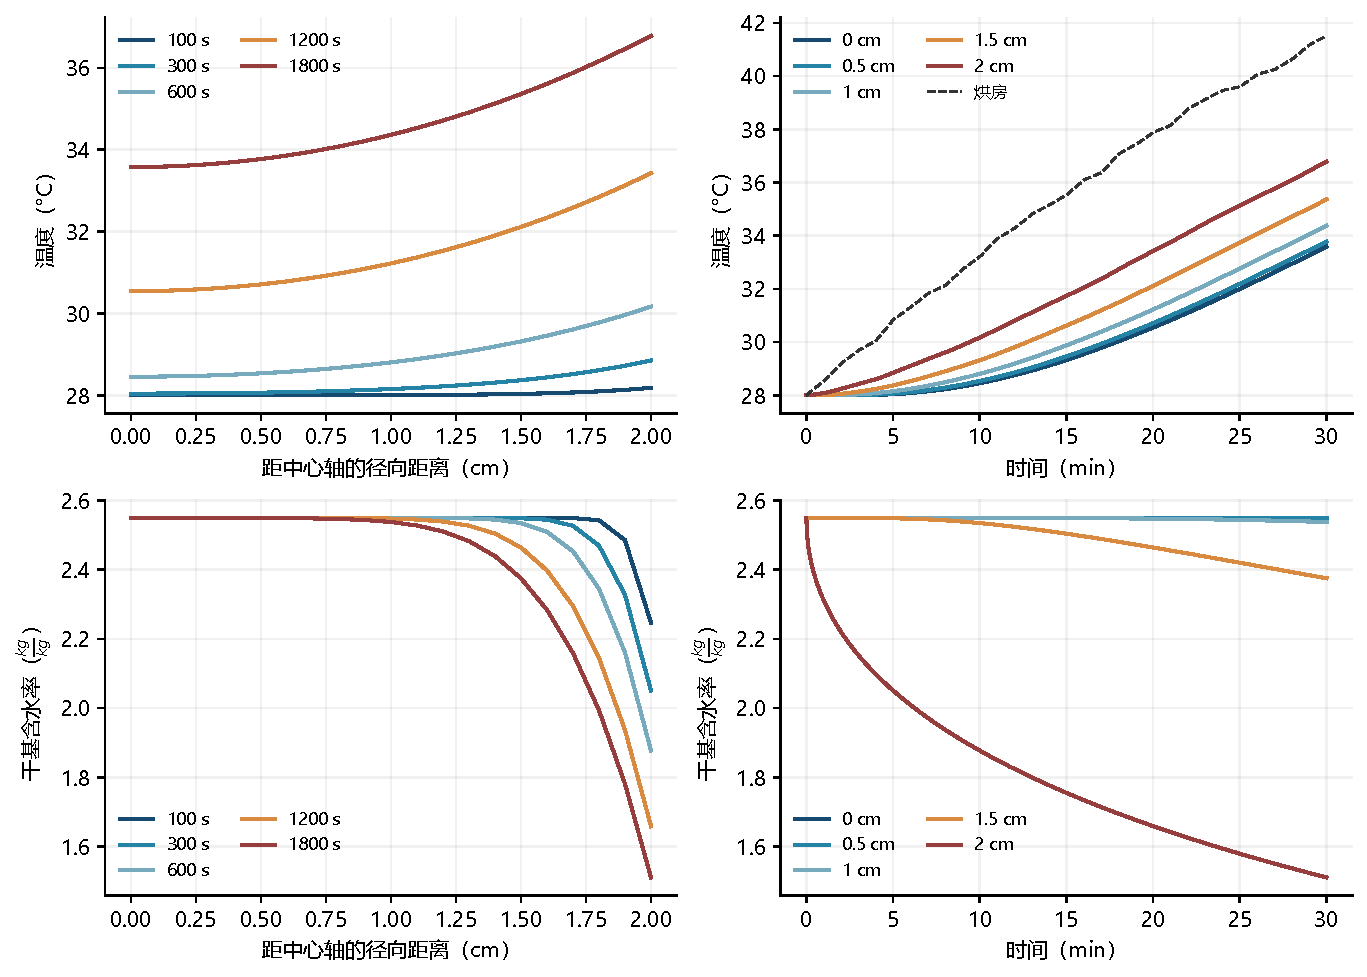
\includegraphics[width=\textwidth]{figures/q1_fields.pdf}
\caption{预热阶段温度与含水率的径向分布及时间变化}
\label{fig:q1-fields}
\end{figure}

图~\ref{fig:q1-fields} 显示，温度变化逐步传至中心，而明显失水仍局限于外层，与热扩散率高于水分扩散系数的量级关系一致。此外，$C$ 减小时 $D(C)$ 随之减小，外层干燥后水分向表面的扩散补给进一步受限。$1800\,\mathrm{s}$ 时，体积加权平均含水率由 $2.5500$ 降至 $2.2936\,\mathrm{kg/kg}$，下降 $10.0566\%$；结合径向差异可知，\textbf{此时药材尚未均匀干燥}。

本问得到的温度与含水率分布回答了预热阶段的时空变化问题。后续在此方程与数值处理框架中引入状态相关物性，可进一步描述全过程的传热传质。


\endgroup
\begingroup
\linespread{1.20}\selectfont
\section{问题二：变物性热湿耦合模型}

\subsection{问题分析}

问题二研究药材在变物性条件下的传热与失水特征，重点给出前三小时内各规定位置的温度和干基含水率。问题一给出了预热阶段的传递基准；本问则从题面初值重新积分，不将 $1800\,\mathrm{s}$ 设为边界切换时刻。这样处理可以在同一环境边界下考察状态相关物性随温度和含水率变化所产生的反馈。

附件~1 的烘房温度和有效水分浓度在相邻采样点之间采用分段线性插值，在 $0$--$10800\,\mathrm{s}$ 内形成连续边界。题面未为本问另行给出换热系数和传质系数，故沿用附录~2 的 $h=25\,\mathrm{W/(m^2\cdot K)}$ 和 $h_m=8\times10^{-7}\,\mathrm{m/s}$ 作为缺参条件下的延续假设。{\heiti\bfseries 药材半径固定为 $R=0.02\,\mathrm{m}$，不考虑收缩、潜热、内部对流及额外热湿源项。}

与问题一中热物性取常数而扩散系数仅随含水率变化的设定相比，本问采用附录~3 的状态相关关系。含水率会同时改变密度、比热容和导热系数，温度与含水率共同决定有效扩散系数，因此需要求解温度场和水分场的联立方程。该模型描述的是题面参数下的变物性有效传递过程，不等同于包含蒸发焓的完整能量模型。

\subsection{模型建立}

取 $r\in[0,R]$ 为到圆柱中心轴的径向距离，$T(r,t)$ 以摄氏度表示，$C(r,t)$ 为干基含水率。在扩散系数的指数项中采用绝对温度 $T_K=T+273.15$，其中 $T_K$ 的单位为 K；除该指数项外，方程和边界中的温度均使用摄氏度数值。附录~3 的状态相关物性写为

\begin{equation}
\begin{aligned}
  \rho(C)&=650+128C,\\[2pt]
  c_p(C)&=1450+2736\frac{C}{C+1},\\[2pt]
  k(C)&=0.21+0.38\frac{C}{C+1},\\[2pt]
  D(C,T)&=2.4\times10^{-3}
  \,\mathrm e^{-\frac{0.45}{C}}
  \,\mathrm e^{-\frac{3850}{T_K}}.
\end{aligned}
\label{eq:q2-properties}
\end{equation}

其中 $\rho$、$c_p$、$k$ 和 $D$ 的单位分别为 $\mathrm{kg/m^3}$、$\mathrm{J/(kg\cdot K)}$、$\mathrm{W/(m\cdot K)}$ 和 $\mathrm{m^2/s}$。由能量守恒和 Fick 型有效扩散得到固定半径下的联立方程

\begin{equation}
\left\{
\begin{aligned}
  \rho(C)c_p(C)\frac{\partial T}{\partial t}
  &=\frac{1}{r}\frac{\partial}{\partial r}
    \left(rk(C)\frac{\partial T}{\partial r}\right),\\
  \frac{\partial C}{\partial t}
  &=\frac{1}{r}\frac{\partial}{\partial r}
    \left(rD(C,T)\frac{\partial C}{\partial r}\right),
  \qquad 0<r<R,\ t>0.
\end{aligned}
\right.
\label{eq:q2-pde}
\end{equation}

\Needspace{14\baselineskip}
完整初边值条件为

\begin{equation}
\left\{
\begin{aligned}
  T(r,0)&=28\,{}^\circ\mathrm{C},\\[2pt]
  C(r,0)&=2.55\,\mathrm{kg/kg},\\[2pt]
  \left.\frac{\partial T}{\partial r}\right|_{r=0}&=0,\\[2pt]
  \left.\frac{\partial C}{\partial r}\right|_{r=0}&=0,\\[2pt]
  -k(C_s)\left.\frac{\partial T}{\partial r}\right|_{r=R}
    &=h\,[T_s-T_\infty(t)],\\[2pt]
  -D(C_s,T_s)\left.\frac{\partial C}{\partial r}\right|_{r=R}
    &=h_m\,[C_s-C_\infty(t)].
\end{aligned}
\right.
\label{eq:q2-ibvp}
\end{equation}

其中 $T_s=T(R,t)$、$C_s=C(R,t)$。对附件~1 中的相邻采样时刻 $t_m$、$t_{m+1}$，令

\begin{equation}
  \lambda(t)=\frac{t-t_m}{t_{m+1}-t_m},\qquad
  \begin{aligned}
  T_\infty(t)&=T_{\infty,m}+\lambda(t)(T_{\infty,m+1}-T_{\infty,m}),\\
  C_\infty(t)&=C_{\infty,m}+\lambda(t)(C_{\infty,m+1}-C_{\infty,m}).
  \end{aligned}
  \label{eq:q2-boundary-interpolation}
\end{equation}

\subsection{模型求解}

对径向区域作均匀离散，温度和水分均采用{\heiti\bfseries 守恒通量离散}，使相邻控制体共用同一界面通量；界面物性取相邻节点的算术平均，圆心按轴对称极限处理，表面施加 Robin 交换条件。空间离散后，采用{\heiti\bfseries BDF 自适应积分}求解温度场和水分场的联立非线性系统。

由于原始含水率变量在非线性内部试探中可能产生非正值，积分器内部采用可逆对数坐标 $z_i=\log C_i$，每次评价时由 $C_i=\mathrm e^{z_i}$ 回到物理方程。该变换只改变数值坐标，不改变含水率的物理定义；解析稀疏 Jacobian 保留温度与含水率之间的交叉依赖。

为分辨初期表面附近的含水率变化，逐级加密径向网格，最终采用 $N=10240$ 个径向区间。{\heiti\bfseries 最终计算}采用相对容差 $10^{-10}$、绝对容差 $10^{-12}$ 和最大内部步长 $2.5\,\mathrm{s}$；按题意每隔 $1\,\mathrm{s}$、每隔 $0.1\,\mathrm{cm}$ 输出，得到每个时刻 $21$ 个径向位置的状态值。每秒输出不代表以 $1\,\mathrm{s}$ 为积分步长，内部步长由误差控制自适应确定。

数值检验覆盖全部规定输出点。空间比较中，$N=5120$ 与 $N=10240$ 的最大差异分别为 $e_T=3.426781\times10^{-6}\,{}^\circ\mathrm{C}$ 和 $e_C=3.731918\times10^{-6}\,\mathrm{kg/kg}$；时间设置收紧后的最大差异分别为 $3.751870\times10^{-6}\,{}^\circ\mathrm{C}$ 和 $4.548273\times10^{-8}\,\mathrm{kg/kg}$。两组加密计算所得六个时刻、五个位置的表值在四位小数下保持一致。上述检验说明离散与积分设置在规定输出上的数值变化已受到控制，但不将其等同于端部、潜热等物理简化误差的消除。

\Needspace{16\baselineskip}
\subsection{结果分析}

规定时刻和规定径向位置的温度见表~\ref{tab:q2-temperature}。表中每隔 $0.5\,\mathrm{h}$ 给出一个时刻，数值由计算解在五个径向位置提取并四舍五入到四位小数。

\begin{table}[H]
  \centering
  \fontsize{10.5pt}{12.6pt}\selectfont
  \renewcommand{\arraystretch}{1.25}
  \captionsetup{font=small,labelfont=bf,textfont=bf}
  \caption{3小时内药材的温度}
  \label{tab:q2-temperature}
  \begin{tabularx}{0.92\textwidth}{|>{\centering\arraybackslash}p{0.23\textwidth}|*{5}{>{\centering\arraybackslash}X|}}
    \hline
    \multirow{2}{*}{时间/h} & \multicolumn{5}{|c|}{到药材中心的距离/cm} \\
    \cline{2-6}
     & 0 & 0.5 & 1 & 1.5 & 2 \\
    \hline
    0.5 & 32.1892 & 32.3821 & 32.9659 & 33.9608 & 35.4130 \\
    \hline
    1.0 & 40.3816 & 40.5536 & 41.0605 & 41.8782 & 42.9976 \\
    \hline
    1.5 & 45.8468 & 45.9348 & 46.1930 & 46.6051 & 47.1400 \\
    \hline
    2.0 & 48.4502 & 48.4881 & 48.5984 & 48.7736 & 49.0033 \\
    \hline
    2.5 & 49.4670 & 49.4792 & 49.5136 & 49.5653 & 49.6609 \\
    \hline
    3.0 & 49.8495 & 49.8553 & 49.8746 & 49.9101 & 49.9664 \\
    \hline
  \end{tabularx}
\end{table}


药材温度呈现由表及里的响应滞后。$0.5\,\mathrm{h}$ 时，中心温度为 $32.1892\,{}^\circ\mathrm{C}$，表面温度为 $35.4130\,{}^\circ\mathrm{C}$，两者相差 $3.2238\,{}^\circ\mathrm{C}$；{\heiti\bfseries 到 $3\,\mathrm{h}$ 时，中心和表面温度分别为 $49.8495$ 和 $49.9664\,{}^\circ\mathrm{C}$，温差缩小到 $0.1169\,{}^\circ\mathrm{C}$。}这说明热扩散在前三小时内逐渐减小早期径向温差。

相同时空位置的干基含水率见表~\ref{tab:q2-moisture}。

\begin{table}[H]
  \centering
  \caption{3 小时内药材的干基含水率（$\mathrm{kg/kg}$）}
  \label{tab:q2-moisture}
  \begin{tabular}{rrrrrr}
    \toprule
    时间/h & $0\,\mathrm{cm}$ & $0.5\,\mathrm{cm}$ & $1\,\mathrm{cm}$ & $1.5\,\mathrm{cm}$ & $2\,\mathrm{cm}$ \\
    \midrule
    0.5 & \resultblank{--} & \resultblank{--} & \resultblank{--} & \resultblank{--} & \resultblank{--} \\
    1.0 & \resultblank{--} & \resultblank{--} & \resultblank{--} & \resultblank{--} & \resultblank{--} \\
    1.5 & \resultblank{--} & \resultblank{--} & \resultblank{--} & \resultblank{--} & \resultblank{--} \\
    2.0 & \resultblank{--} & \resultblank{--} & \resultblank{--} & \resultblank{--} & \resultblank{--} \\
    2.5 & \resultblank{--} & \resultblank{--} & \resultblank{--} & \resultblank{--} & \resultblank{--} \\
    3.0 & \resultblank{--} & \resultblank{--} & \resultblank{--} & \resultblank{--} & \resultblank{--} \\
    \bottomrule
  \end{tabular}
\end{table}



水分梯度比温度梯度保持得更久。{\heiti\bfseries $3\,\mathrm{h}$ 时，中心含水率为 $1.7662\,\mathrm{kg/kg}$，表面含水率为 $1.0081\,\mathrm{kg/kg}$，径向差为 $0.7581\,\mathrm{kg/kg}$。}相对于初始值，中心和表面含水率分别下降约 $30.74\%$ 和 $60.47\%$，表明表面已明显失水而中心仍较湿，平均含水率或表面值不能替代全域状态。

为比较空间分布与时间响应，图~\ref{fig:q2-fields} 给出温度和含水率的径向剖面及代表位置的时间曲线。

\begin{figure}[H]
  \centering
  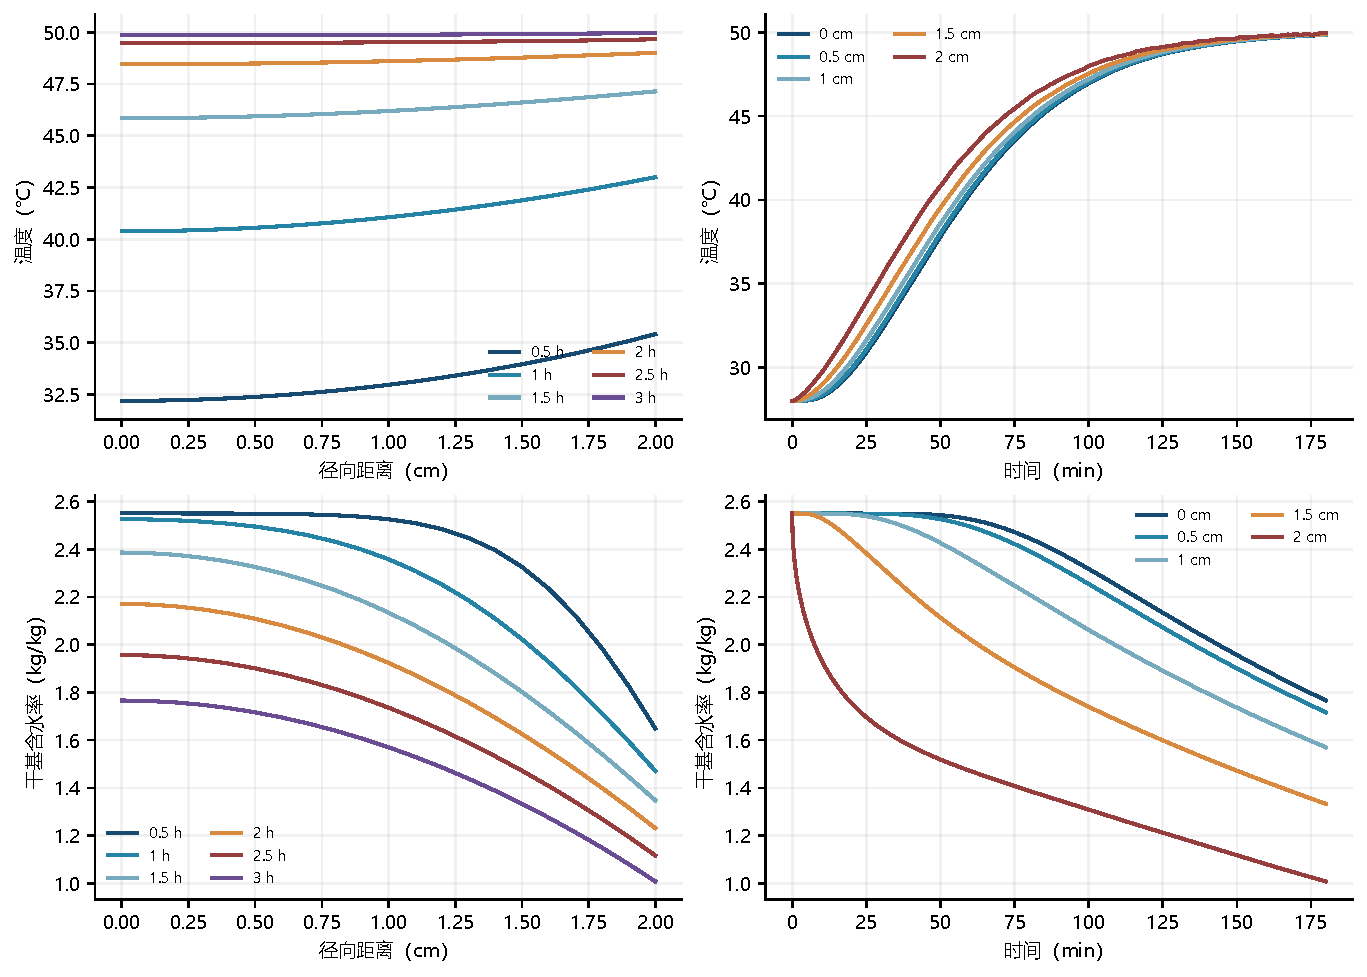
\includegraphics[width=\textwidth]{figures/q2_fields.pdf}
  \caption{问题二温度与干基含水率的径向剖面及时间演化。左列为 $0.5$、$1$、$1.5$、$2$、$2.5$、$3\,\mathrm{h}$ 六个时刻的径向剖面，右列为 $0$、$0.5$、$1$、$1.5$、$2\,\mathrm{cm}$ 五个位置的时间曲线。}
  \label{fig:q2-fields}
\end{figure}

图~\ref{fig:q2-fields} 显示，温度剖面先由表面向内推进，含水率剖面则始终表现为由中心向表面递减的梯度。扩散系数中的温度因子随 $T$ 增大而提高局部 $D$，而含水率降低会使 $\mathrm e^{-\frac{0.45}{C}}$ 变小；两种状态作用共同决定表层与内部之间的水分迁移。初始状态下 $D=5.642\times10^{-9}\,\mathrm{m^2/s}$，$3\,\mathrm{h}$ 时中心和表面的局部值约为 $1.239\times10^{-8}$ 和 $1.027\times10^{-8}\,\mathrm{m^2/s}$。这些数值反映的是状态相关的有效扩散系数，不能单独推出整个药材的水分迁移速率必然加快或减慢。

为展示温度场和含水率场在整个计算窗口内的时空演化，图~\ref{fig:q2-spacetime} 给出 $0$--$3\,\mathrm{h}$、$0$--$2\,\mathrm{cm}$ 范围内的两幅时空曲面。温度曲面随时间整体升高，后期沿径向逐渐趋平；含水率曲面在初期靠近表面处下降较快，内部仍保持较高含水率，随后失水区域向中心推进，至 $3\,\mathrm{h}$ 仍保留明显的径向差异。

\begin{figure}[H]
  \centering
  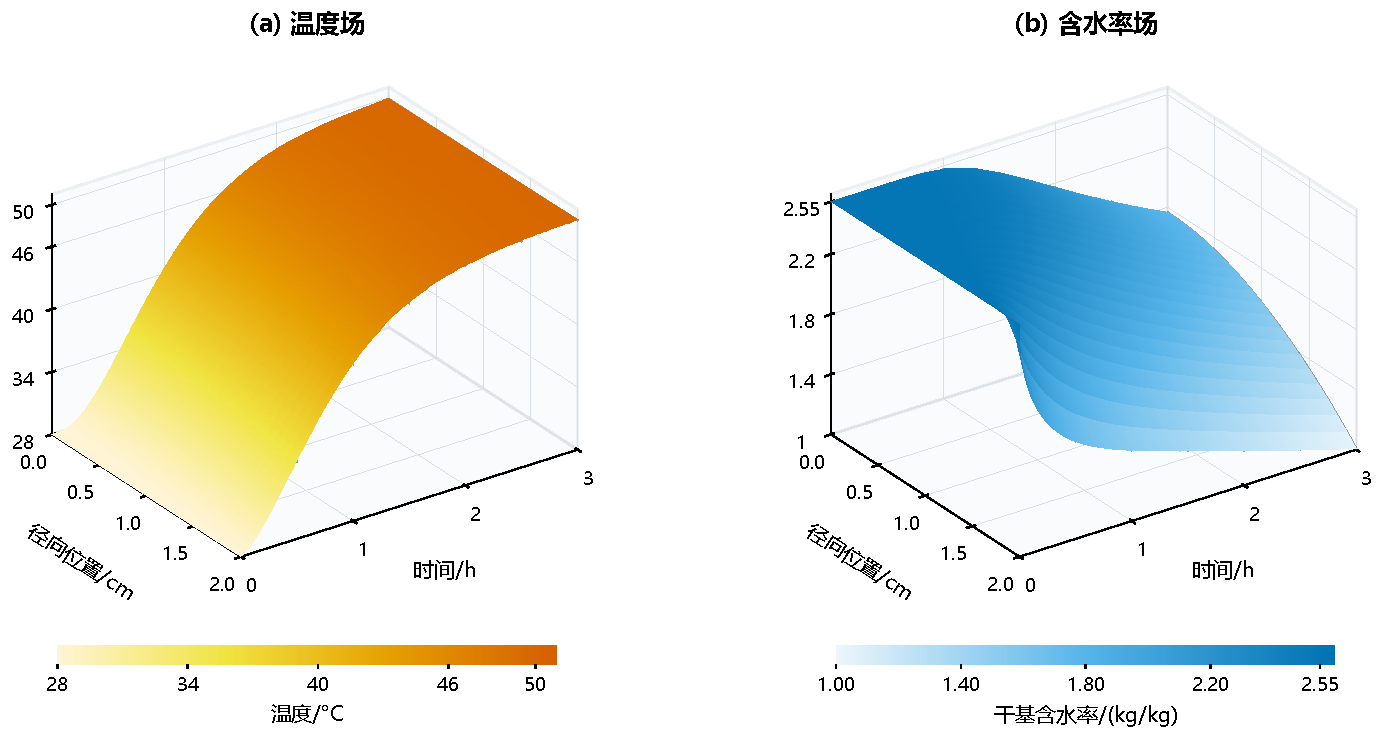
\includegraphics[width=\textwidth]{figures/q2_spacetime.pdf}
  \caption{问题二温度场与干基含水率场的时空演化曲面。横轴为时间，纵轴为径向位置，时间范围为 $0$--$3\,\mathrm{h}$，径向范围为 $0$--$2\,\mathrm{cm}$。}
  \label{fig:q2-spacetime}
\end{figure}

为考察表面交换系数对结果的影响，$h_m$ 降低 $20\%$ 时，$3\,\mathrm{h}$ 时中心和表面含水率相对基准分别增加约 $5.21\%$ 和 $16.80\%$；提高 $20\%$ 时，分别减少约 $4.20\%$ 和 $13.34\%$。$h$ 降低 $20\%$ 时，中心和表面含水率分别增加约 $0.59\%$ 和 $0.15\%$；提高 $20\%$ 时，分别减少约 $0.37\%$ 和 $0.14\%$。在所考察的扰动范围内，含水率对传质系数的变化更为敏感。

为检验上述结果与问题一的衔接，在共同初值、边界、半径以及 $0$--$1800\,\mathrm{s}$ 时间范围内进行逐点比较。问题一在 $1800\,\mathrm{s}$ 时中心和表面温度分别为 $33.5753$ 和 $36.7856\,{}^\circ\mathrm{C}$，问题二分别为 $32.1892$ 和 $35.4130\,{}^\circ\mathrm{C}$，对应低 $1.3861$ 和 $1.3725\,{}^\circ\mathrm{C}$。在水分场，表面含水率由问题一的 $1.5102\,\mathrm{kg/kg}$ 变为问题二的 $1.6486\,\mathrm{kg/kg}$，而 $r=1.5\,\mathrm{cm}$ 处由 $2.3755\,\mathrm{kg/kg}$ 变为 $2.3257\,\mathrm{kg/kg}$。两个模型均表现为表面先升温、失水，中心响应滞后，给出一致的定性趋势。

这种差异与初始物性尺度相符：问题一的体积热容为 $2.132\times10^{6}\,\mathrm{J/(m^3\cdot K)}$、热扩散率为 $1.6886\times10^{-7}\,\mathrm{m^2/s}$，问题二分别为 $3.334695\times10^{6}\,\mathrm{J/(m^3\cdot K)}$ 和 $1.4483\times10^{-7}\,\mathrm{m^2/s}$，初始升温响应因而更具热惯性；初始扩散系数则分别为 $4.9377\times10^{-9}$ 和 $5.6417\times10^{-9}\,\mathrm{m^2/s}$。两问采用不同本构关系，故该对照用于解释预测差异，而不作为精度优劣的判据。{\heiti\bfseries 问题二更适合描述持续升温、失水过程中局部物性反馈的影响。}

% Keep the following question heading together with its opening analysis.
\par\Needspace{9\baselineskip}

\endgroup
\section{问题三：烘干时间}

\subsection{问题分析}

第三问要求确定药材各处含水率均低于 $0.15\,\mathrm{kg/kg}$ 的烘干时间。该问与第二问具有相同的几何、物性关系和热湿耦合方程，因此沿用式~\eqref{eq:q2-pde}、\eqref{eq:q2-ibvp}，将计算时间延长至满足干燥要求。由于内部失水滞后于表面，\textbf{终止条件应由全域最大含水率确定}。

附件~1 给出的环境数据覆盖前 $4\,\mathrm h$。最后一小时的温度和环境水分浓度均值分别为 $49.9989\,{}^\circ\mathrm C$ 和 $0.0499875\,\mathrm{kg/kg}$，说明观测末段已经接近题设稳定工况。据此，前 $4\,\mathrm h$ 继续采用附件数据的分段线性插值，此后取

\begin{equation}
  T_\infty=50\,{}^\circ\mathrm C,\qquad
  C_\infty=0.05\,\mathrm{kg/kg}.
  \label{eq:q3-long-boundary}
\end{equation}

式~\eqref{eq:q3-long-boundary} 是第三问的长期边界条件，后文给出的烘干时间均以该工况持续保持为前提。

\subsection{终点判定}

记药材内部最大含水率为 $M(t)$，临界烘干时间 $t_d$ 定义为

\begin{equation}
  \left\{
  \begin{aligned}
    M(t)&=\max_{0\le r\le R_0}C(r,t),\\
    t_d&=\inf\left\{t\ge0:M(t)\le0.15\right\}.
  \end{aligned}
  \right.
  \label{eq:q3-end-time}
\end{equation}

其中 $R_0=0.02\,\mathrm m$，$C$ 的单位为 $\mathrm{kg/kg}$。临界状态满足 $M(t_d)=0.15$；继续干燥后，药材各处含水率严格低于阈值。

计算结果显示，在整个烘干过程中，药材含水率均由圆心向表面逐渐降低，最大含水率始终出现在圆心。因此，\textbf{圆心是最后达到干燥要求的位置}，式~\eqref{eq:q3-end-time} 可进一步化为

\begin{equation}
  M(t)=C(0,t),\qquad C(0,t_d)=0.15.
  \label{eq:q3-center-event}
\end{equation}

\subsection{模型求解}

沿用第二问的守恒空间离散和 BDF 自适应积分，联立推进温度场与含水率场。在积分过程中监测

\[
  g(t)=C(0,t)-0.15
\]

的首次下降过零，并利用连续插值定位 $t_d$。随后以全域最大含水率复核终点，确认临界点前尚未全部达标，临界点后已严格低于阈值。完整结果按 $60\,\mathrm s$ 的时间间隔和 $0.1\,\mathrm{cm}$ 的空间间隔保存，论文结果表的末行直接取临界状态。

\subsection{结果分析}

在 $4\,\mathrm h$ 后持续满足式~\eqref{eq:q3-long-boundary} 的条件下，药材全域含水率首次达到规定阈值的时间为

\[
  \boxed{t_d\approx57.4722\,\mathrm h}.
\]

该数值按题目要求保留四位小数。每隔 $6\,\mathrm h$ 及临界时刻的含水率见表~\ref{tab:q3-moisture}。

\begin{table}[H]
  \centering
  \caption{药材烘干过程的水分浓度（$\mathrm{kg/kg}$）}
  \label{tab:q3-moisture}
  \begin{tabular}{rrrrrr}
    \toprule
    时间/h & $0\,\mathrm{cm}$ & $0.5\,\mathrm{cm}$ & $1\,\mathrm{cm}$ & $1.5\,\mathrm{cm}$ & $2\,\mathrm{cm}$ \\
    \midrule
    6       & 1.0170 & 0.9881 & 0.9015 & 0.7550 & 0.5328 \\
    12      & 0.4561 & 0.4432 & 0.4031 & 0.3297 & 0.1642 \\
    18      & 0.2988 & 0.2915 & 0.2687 & 0.2253 & 0.0845 \\
    24      & 0.2378 & 0.2327 & 0.2167 & 0.1855 & 0.0665 \\
    30      & 0.2058 & 0.2018 & 0.1892 & 0.1641 & 0.0598 \\
    36      & 0.1859 & 0.1825 & 0.1718 & 0.1504 & 0.0566 \\
    42      & 0.1721 & 0.1691 & 0.1597 & 0.1407 & 0.0549 \\
    48      & 0.1618 & 0.1592 & 0.1507 & 0.1334 & 0.0537 \\
    54      & 0.1539 & 0.1514 & 0.1436 & 0.1277 & 0.0530 \\
    57.4722 & 0.1500 & 0.1477 & 0.1402 & 0.1249 & 0.0527 \\
    \bottomrule
  \end{tabular}
\end{table}


临界时刻，圆心含水率为 $0.1500\,\mathrm{kg/kg}$，表面已降至 $0.0527\,\mathrm{kg/kg}$。表面约在 $12.55\,\mathrm h$ 达到阈值，圆心则在 $57.47\,\mathrm h$ 最后达标，两者相差约 $44.92\,\mathrm h$。可见，表面含水率较早降至阈值时，药材内部仍未满足烘干要求，因而\textbf{表面状态不能代表药材整体的干燥程度，实际停机时刻应由圆心含水率确定}。

\subsection{结果可靠性检验}

临界烘干时间是本问的核心结果。为考察其是否依赖径向网格的划分尺度，在其余条件不变的情况下，分别取 2560、5120 和 10240 个径向区间进行计算，结果见表~\ref{tab:q3-convergence}。

\begin{table}[H]
  \centering
  \fontsize{10.5pt}{12.6pt}\selectfont
  \renewcommand{\arraystretch}{1.25}
  \captionsetup{font=small,labelfont=bf,textfont=bf}
  \caption{临界烘干时间的网格收敛}
  \label{tab:q3-convergence}
  \begin{tabularx}{0.82\textwidth}{|>{\centering\arraybackslash}X|>{\centering\arraybackslash}X|>{\centering\arraybackslash}X|>{\centering\arraybackslash}X|}
    \hline
    网格等级 & 区间数 $N$ & 达标时间/h & 相邻差异/s \\
    \hline
    粗 & 2560  & 57.471395 & --- \\
    \hline
    中 & 5120  & 57.472066 & 2.42 \\
    \hline
    细 & 10240 & 57.472244 & 0.64 \\
    \hline
  \end{tabularx}
\end{table}


由表可见，网格逐级加密时，临界烘干时间趋于稳定，其中 5120 个区间加密至 10240 个区间后，终点仅变化 $0.64\,\mathrm s$。在细网格上进一步收紧时间积分容差并减小最大步长，所得终点又仅变化 $0.0129\,\mathrm s$。空间和时间两方面的比较均表明，\textbf{现有离散精度足以支撑 $57.4722\,\mathrm h$ 的终点判断}。此外，含水率总量变化与表面传质通量之间的最大相对平衡残差为 $5.32\times10^{-7}$，说明离散求解较好地保持了质量守恒。

\subsection{长期工况敏感性}

由于超过九成的预测时段位于环境观测窗口之外，长期边界是影响终点解释的重要假设。保持前 $4\,\mathrm h$ 的附件数据不变，只改变此后的恒定工况，结果见图~\ref{fig:q3-boundary-sensitivity}。

\begin{figure}[H]
  \centering
  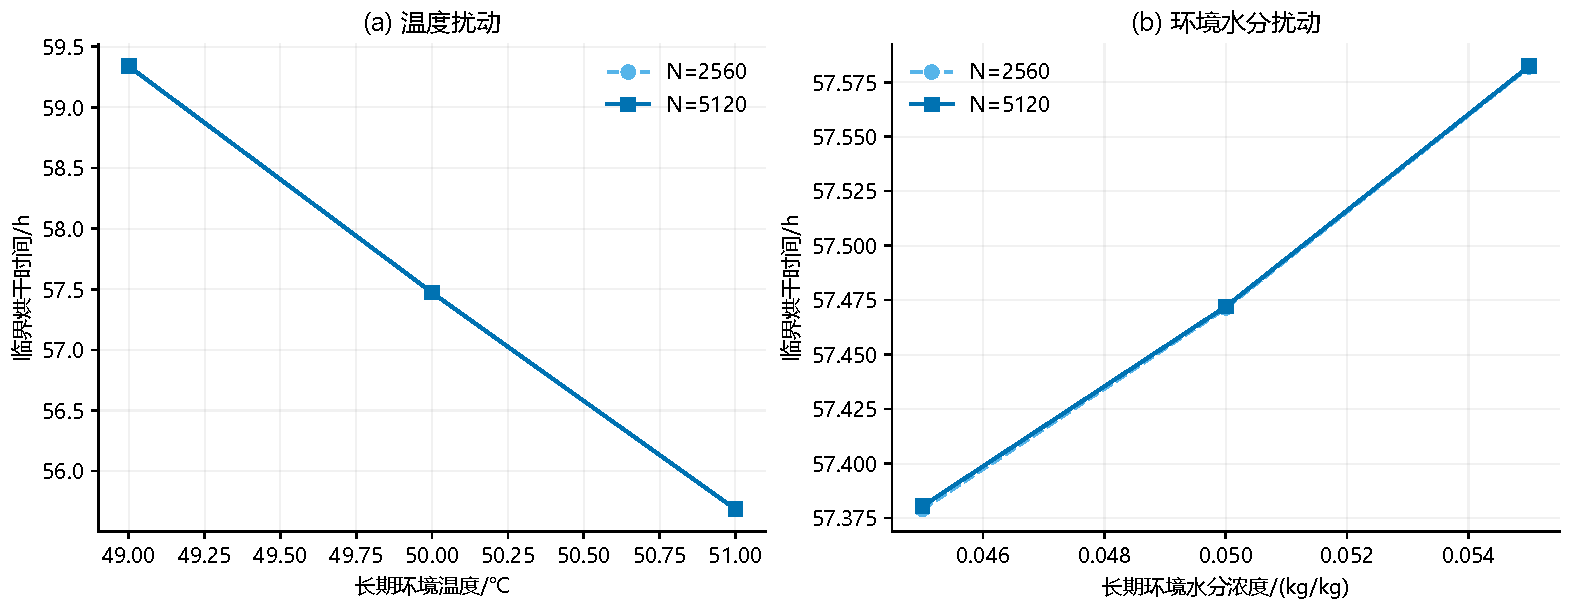
\includegraphics[width=0.96\textwidth]{figures/q3_boundary_sensitivity.pdf}
  \caption{长期环境条件对临界烘干时间的影响}
  \label{fig:q3-boundary-sensitivity}
\end{figure}

长期温度取 $49$、$50$ 和 $51\,{}^\circ\mathrm C$ 时，临界时间分别为 $59.3392$、$57.4721$ 和 $55.6865\,\mathrm h$；相对基准工况，温度降低 $1\,{}^\circ\mathrm C$ 使烘干时间延长 $1.867\,\mathrm h$，温度升高 $1\,{}^\circ\mathrm C$ 则使其缩短 $1.786\,\mathrm h$。当环境水分浓度取 $0.045$、$0.050$ 和 $0.055\,\mathrm{kg/kg}$ 时，临界时间分别为 $57.3804$、$57.4721$ 和 $57.5824\,\mathrm h$，变化约为 $-0.09$ 至 $0.11\,\mathrm h$。

因此，在所考察的扰动范围内，\textbf{温度变化造成的终点偏移明显大于环境水分浓度变化}，表明最终达标时间对这组长期温度扰动更敏感。这进一步说明，$57.4722\,\mathrm h$ 是长期环境维持基准工况时的条件预测，而不是脱离运行条件的固定时长。图中的扰动范围用于比较给定工况，不代表未来环境的统计置信区间。

\subsection{后期干燥长尾的形成}

为解释圆心达标明显滞后的原因，将各时刻的温度和含水率代入扩散系数关系，得到圆心、$r=0.5R_0$ 和表面的有效扩散系数变化，如图~\ref{fig:q3-diffusivity} 所示。

\begin{figure}[H]
  \centering
  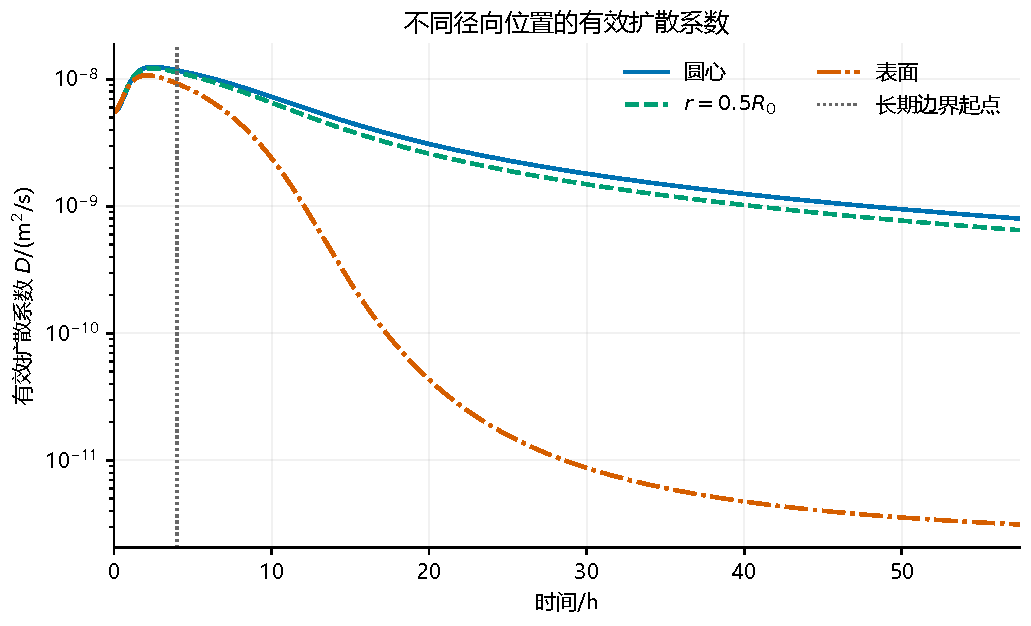
\includegraphics[width=0.86\textwidth]{figures/q3_diffusivity.pdf}
  \caption{不同径向位置的有效扩散系数随时间的变化}
  \label{fig:q3-diffusivity}
\end{figure}

图~\ref{fig:q3-diffusivity} 显示，升温初期三个位置的扩散系数均有所增大；温度逐渐稳定后，含水率下降的影响开始占据主导，扩散系数随之减小。由于表层最先失水，其扩散系数也最早、最快下降，并逐渐与内部曲线拉开差距。到临界时刻，圆心和表面的扩散系数分别约为 $8.00\times10^{-10}\,\mathrm{m^2/s}$ 和 $3.12\times10^{-12}\,\mathrm{m^2/s}$，前者约为后者的 256 倍。

这说明药材在后期并非均匀干燥：外层含水率降低后，逐渐形成扩散能力较弱的区域，而圆心附近仍保留较多水分。内部水分向外迁移时需要经过这一低扩散区域，使后期失水速度不断减缓。因此，表面在 $12.55\,\mathrm h$ 达标后，圆心仍需较长时间才能降至阈值，最终形成从 $12.55\,\mathrm h$ 延续至 $57.47\,\mathrm h$ 的干燥长尾。\textbf{第三问较长的终点时间，反映的正是内部剩余水分缓慢向外迁移的过程。}这里的 256 倍用于说明扩散能力的径向差异；实际传质速率仍由扩散系数和含水率梯度共同决定。

\section{问题四：考虑收缩的移动边界模型}

本问在第~\ref{sec:model-preparation} 节的传递定律基础上，进一步引入附件~2 的半径变化及附录~4 的物性关系。输运方程、表面交换和空间积分须与变化区域相适应。

\subsection{移动区域与归一化坐标}

附件~2 给出药材半径 $R(t)$。为避免随时间重新划分物理网格，引入固定计算坐标

\begin{equation}
  \xi=\frac{r}{R(t)},\qquad 0\le \xi\le 1.
  \label{eq:q4-xi}
\end{equation}

对任意状态 $F(r,t)=\widetilde F(\xi,t)$，坐标变换满足

\begin{equation}
  \left.\frac{\partial F}{\partial t}\right|_r
  =\left.\frac{\partial \widetilde F}{\partial t}\right|_\xi
  -\frac{\dot R(t)}{R(t)}\xi
  \frac{\partial \widetilde F}{\partial \xi},
  \qquad
  \frac{\partial F}{\partial r}
  =\frac{1}{R(t)}\frac{\partial \widetilde F}{\partial \xi}.
  \label{eq:q4-transform}
\end{equation}

式~\eqref{eq:q4-transform} 只给出坐标恒等关系；最终方程还必须与干基含水率的质量守恒口径一致。不能只把问题三程序中的 $R_0$ 替换为 $R(t)$。

\subsection{问题四物性参数}

附录~4 给出的经验公式为

\begin{align}
  \rho(C)&=760+90C, \\
  c_p(C)&=1850+2150\frac{C}{C+1}, \\
  k(C)&=0.12+0.20\frac{C}{C+1}, \\
  D(C,T)&=4.2\times10^{-4}
  \exp\left(-\frac{0.30}{C}\right)
  \exp\left(-\frac{3850}{T}\right),
  \qquad T\text{ 取 K}.
  \label{eq:q4-properties}
\end{align}

移动边界方程、表面通量和体积积分均在 $R(t)$ 下重写。半径数据在采样点之间采用\resultblank{单调插值或分段插值方法}，并对 $\dot R(t)$ 的数值稳定性进行检查。

\subsection{区分收缩效应与物性变化}

问题三采用附录~3，问题四采用附录~4，同时问题四还加入 $R(t)$。为了避免把两种变化混在一起，设置表~\ref{tab:q4-controls} 的 $2\times2$ 对照。

\begin{table}[H]
  \centering
  \caption{问题四的控制变量对照设计}
  \label{tab:q4-controls}
  \begin{tabular}{ccc}
    \toprule
    方案 & 半径 & 物性经验公式 \\
    \midrule
    A & 固定 $R_0$ & 附录~3 \\
    B & 变化 $R(t)$ & 附录~3 \\
    C & 固定 $R_0$ & 附录~4 \\
    D & 变化 $R(t)$ & 附录~4 \\
    \bottomrule
  \end{tabular}
\end{table}

其中 A 对应问题三主结果，D 对应问题四主结果；A 与 B 的差异用于观察几何收缩影响，A 与 C 的差异用于观察物性公式变化，四组联合用于检查二者的交互作用。该对照属于补充数值实验，应与题目规定的主结果分开呈现。

\subsection{终止条件与结果}

移动区域下定义

\begin{equation}
  C_{\max}^{(s)}(t)=\max_{0\le \xi\le1}\widetilde C(\xi,t),
  \qquad
  t_{\mathrm{end}}^{(s)}=\inf\left\{t>0:C_{\max}^{(s)}(t)<0.15\right\}.
  \label{eq:q4-end-time}
\end{equation}

\begin{table}[H]
  \centering
  \caption{考虑收缩时烘干过程的干基含水率（$\mathrm{kg/kg}$）}
  \label{tab:q4-moisture}
  \begin{tabular}{rrrrrr}
    \toprule
    时间/h & $0\,\mathrm{cm}$ & $0.5\,\mathrm{cm}$ & $1\,\mathrm{cm}$ & $\cdots$ & 药材表面 \\
    \midrule
    6  & \resultblank{--} & \resultblank{--} & \resultblank{--} & \resultblank{--} & \resultblank{--} \\
    12 & \resultblank{--} & \resultblank{--} & \resultblank{--} & \resultblank{--} & \resultblank{--} \\
    18 & \resultblank{--} & \resultblank{--} & \resultblank{--} & \resultblank{--} & \resultblank{--} \\
    $\vdots$ & $\vdots$ & $\vdots$ & $\vdots$ & $\vdots$ & $\vdots$ \\
    $t_{\mathrm{end}}^{(s)}$ & \resultblank{--} & \resultblank{--} & \resultblank{--} & \resultblank{--} & \resultblank{--} \\
    \bottomrule
  \end{tabular}
\end{table}


表中固定位置按 $0.5\,\mathrm{cm}$ 间隔列到当前表面以内，并单独给出实时表面值；超出当前药材区域的位置不做空间外推。最终列数和表头以附件~3 的 \texttt{result4.xlsx} 模板为准。

\placeholderfigure{建议同时展示半径曲线、归一化坐标下的含水率剖面，以及四组控制实验的达标时刻。}{尺寸收缩及物性变化对烘干过程的影响}

考虑收缩后，药材烘干时长为\resultblank{数值}\,h。相对于固定半径基准，纯几何收缩、物性公式变化及其组合的影响分别为\resultblank{对照结果与单位}。

\draftnote{只有完成控制变量对照后，才能把某部分时长变化解释为收缩效应。若附件仅给半径而没有长度变化，应明确体积、密度和干物质守恒如何同时处理。}

\subsection{本问小结}

本问利用归一化坐标把求解区域固定到 $[0,1]$，生成 \texttt{result4.xlsx}，并通过对照实验解释尺寸变化与经验物性的独立影响。

\section{模型验证与敏感性分析}

验证围绕本题的具体失效风险设计，不用“曲线平滑”替代正确性检查。

\subsection{离散精度与收敛}

分别改变径向网格数 $N_r$ 和内部时间步 $\Delta t$，比较题面指定节点、最大含水率和烘干终点。以加密前后的终点相对变化

\begin{equation}
  \varepsilon_t=
  \frac{\left|t_{\mathrm{end}}^{\mathrm{fine}}-t_{\mathrm{end}}^{\mathrm{base}}\right|}
  {t_{\mathrm{end}}^{\mathrm{fine}}}
  \label{eq:convergence}
\end{equation}

作为主要收敛指标，并给出\resultblank{预先确定的容许标准}。

\subsection{初边值与守恒检查}

\begin{enumerate}
  \item $t=0$ 时所有径向节点应恢复题面初值；$r=0$ 的数值梯度应满足中心对称条件。
  \item 表面离散通量应与对流边界的热量或水分交换量一致，符号方向不得相反。
  \item 对含水率场进行体积积分，比较内部总水分变化与表面累计传质通量。问题四应使用随 $R(t)$ 变化的体积元。
  \item 每个 Excel 的时间列、空间列、单位、工作表名称和四位小数格式必须与附件~3 模板一致。
\end{enumerate}

\subsection{物理合理性检查}

检查温度是否超出边界与初值能够支持的范围，含水率是否出现负值或非物理振荡，材料参数是否始终位于正值范围。若温度或含水率并非单调变化，应回到附件边界和通量方向解释，不能直接删除异常点。

\subsection{关键参数敏感性}

优先选择传质系数 $h_m$、扩散系数经验式和烘房恒温值等直接控制干燥速率的量。对参数 $p$ 进行规定比例扰动，使用无量纲敏感度

\begin{equation}
  S_p=\frac{\Delta t_{\mathrm{end}}/t_{\mathrm{end}}}
  {\Delta p/p}
  \label{eq:sensitivity}
\end{equation}

比较其对烘干时长的影响。若题面没有给出参数的统计误差分布，相关结果称为“情景敏感性”，不解释为置信区间。

\begin{table}[H]
  \centering
  \caption{验证项目及最终证据位置}
  \label{tab:validation-contracts}
  \begin{tabularx}{\textwidth}{p{0.22\textwidth}Xp{0.22\textwidth}}
    \toprule
    验证项目 & 判定内容 & 证据位置 \\
    \midrule
    网格和时间步收敛 & 指定输出与达标时刻是否稳定 & \resultblank{图/表编号} \\
    初始与边界条件 & 初值、中心梯度、表面通量是否满足 & \resultblank{结果文件} \\
    水分平衡 & 内部水分变化与累计表面通量残差 & \resultblank{图/表编号} \\
    阈值首次穿越 & 终点前未达标、终点后全部达标 & \resultblank{图/表编号} \\
    Excel 格式契约 & 行列、单位、表名和精度符合模板 & \resultblank{校验日志} \\
    \bottomrule
  \end{tabularx}
\end{table}


\section{模型评价与推广}

\subsection{模型优势}

最终稿应结合实际完成情况评价以下方面：四问是否共享同一套状态和边界口径；变系数是否以通量形式保留；达标时刻是否由空间最大含水率首次穿越确定；问题四是否通过移动坐标与控制变量对照解释收缩影响。

\draftnote{只保留已由方程、代码和验证结果支持的优点。不要使用“精度很高”“适用性强”等没有证据的表述。}

\subsection{模型局限}

本题可能的主要局限包括：一维径向近似忽略端面和轴向差异；附件中的环境量未必等同于药材表面平衡含水率；经验物性公式的适用范围有限；半径曲线不能完整描述长度、孔隙率和组织结构变化。最终稿应说明哪些局限已经通过对照或敏感性分析评估，哪些仍构成结论边界。

\subsection{模型推广}

在获得其他药材的几何、平衡含水率、传热传质系数和物性参数后，本文的固定区域与移动区域框架可用于比较不同烘干条件下的内部均匀性和达标时长。若用于实际工艺优化，还需要加入能耗、有效成分保持率和实验标定数据，不能仅凭本题仿真直接给出生产参数。

\subsection{主要结论}

\begin{enumerate}
  \item 问题一：\resultblank{预热阶段最重要的温度与含水率结论}。
  \item 问题二：\resultblank{变物性全过程最重要的机制结论}。
  \item 问题三：固定半径条件下烘干时长为\resultblank{数值与单位}。
  \item 问题四：考虑收缩后的烘干时长为\resultblank{数值与单位}，收缩和物性变化的影响分别为\resultblank{对照结论}。
\end{enumerate}



\newpage
\section*{参考文献}
\addcontentsline{toc}{section}{参考文献}

% 只加入正文实际引用且已核验的真实文献。下面是格式示例，使用时取消注释并替换。
% \begin{thebibliography}{99}
%   \bibitem{ref-drying} 作者. 题名[J]. 期刊名, 年份, 卷(期): 页码.
%   \bibitem{ref-numerical} Author. Title[M]. Publisher, year.
% \end{thebibliography}

\draftnote{尚未加入参考文献。最终稿中每条文献必须真实存在、正文实际引用，并核对作者、题名、年份和页码。}



\newpage
\section*{附录 A\quad 核心代码与文件说明}
\addcontentsline{toc}{section}{附录 A 核心代码与文件说明}

最终支撑材料建议按下列模块组织：

\begin{table}[H]
  \centering
  \caption{代码与输出文件对应关系}
  \begin{tabularx}{\textwidth}{p{0.25\textwidth}Xp{0.25\textwidth}}
    \toprule
    建议文件 & 功能 & 主要输出 \\
    \midrule
    \texttt{data\_io.py} & 附件读取、单位转换、插值和模板写入 & 清洗后的边界与半径数据 \\
    \texttt{solver\_fixed.py} & 问题一至三的固定区域热湿求解器 & 时空状态数组 \\
    \texttt{solver\_shrink.py} & 问题四的归一化坐标和移动边界求解器 & 收缩域时空状态数组 \\
    \texttt{event\_time.py} & 空间最大含水率与首次达标事件 & 烘干时长 \\
    \texttt{validate.py} & 收敛、边界、守恒和 Excel 格式检查 & 校验报告 \\
    \texttt{make\_figures.py} & 从同源结果数据生成论文图表 & \texttt{figures/} \\
    \bottomrule
  \end{tabularx}
\end{table}

\draftnote{本模板暂不嵌入虚构代码。实现完成后只选取能够说明核心离散、边界处理和终点判断的片段；完整代码随支撑材料提交。}

% 示例：代码存在后取消注释。
% \lstinputlisting[language=Python,caption={固定区域求解器核心函数}]{../code/solver_fixed.py}


\end{document}
